\documentclass[11pt,pdftex,letterpaper]{article}
\usepackage[
    hdivide={1in,*,1in},
    vdivide={1in,*,1in},
]{geometry}

\usepackage{graphicx}
\usepackage{fancyhdr}
\pagestyle{fancy}
\usepackage{listings}
\usepackage{lastpage}
\usepackage{xcolor}
\usepackage{amsmath}

\colorlet{punctuationColor_}{red!60!black}
\definecolor{backgroundColor_}{HTML}{EEEEEE}
\definecolor{delimiterColor_}{RGB}{20,105,176}

\newcommand{\mytilde}{\raise.17ex\hbox{$\scriptstyle\mathtt{\sim}$}}

\lstdefinelanguage{txt}{
    basicstyle=\normalfont\ttfamily,
    numbers=left,
    numberstyle=\scriptsize,
    stepnumber=1,
    numbersep=8pt,
    showstringspaces=false,
    breaklines=true,
    frame=lines,
    backgroundcolor=\color{backgroundColor_},
    literate=
      {:}{{{\color{punctuationColor_}{:}}}}{1}
      {,}{{{\color{punctuationColor_}{,}}}}{1}
      {\{}{{{\color{delimiterColor_}{\{}}}}{1}
      {\}}{{{\color{delimiterColor_}{\}}}}}{1}
      {[}{{{\color{delimiterColor_}{[}}}}{1}
      {]}{{{\color{delimiterColor_}{]}}}}{1},
}

\setlength{\topmargin}{-.5in}
\setlength{\textheight}{9in}
\setlength{\oddsidemargin}{.125in}
\setlength{\textwidth}{6.25in}
\setlength{\headheight}{14pt}

\rhead{\thepage\ of \pageref{LastPage}}
\cfoot{\small{Boys Town National Research Hospital - Technology Core}}

\begin{document}
\vspace*{30ex}
\begin{center}
\textbf{AV Speech in Noise 3.4.0}
\end{center}
\pagebreak
\tableofcontents
\pagebreak

\section{Test Setup}
The application opens to the test setup window shown in Figure~\ref{fig:test-setup-window}.
\begin{figure}
	\centering
	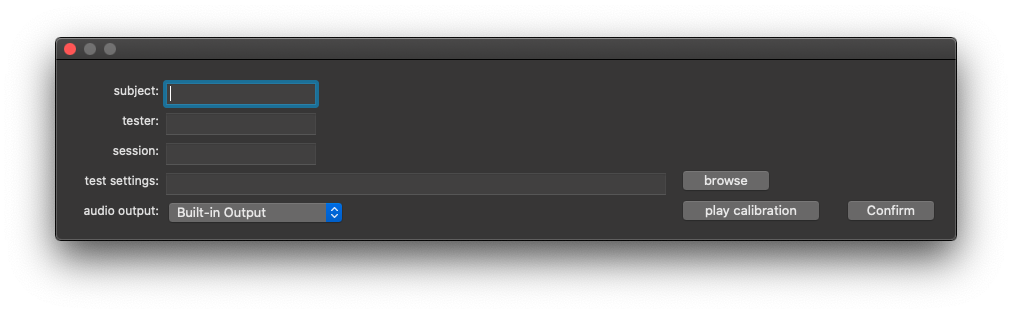
\includegraphics[width = 0.9\linewidth]{test-setup-window.png}
	\caption{test setup window}
	\label{fig:test-setup-window}
\end{figure}
The tester browses for \texttt{test settings}, a plaintext file used for test configuration. An example is shown in Listing~\ref{lst:example-test-settings}.

\noindent\begin{minipage}{\textwidth}
	\lstinputlisting[
	language=txt,
	label={lst:example-test-settings},
	caption={example test settings file}
	]{example-settings.txt}
\end{minipage}
Each setting is printed on its own line. The order of settings does not matter. The following describes each setting.
\subsection{targets}
\texttt{targets} specifies a directory containing audio and/or video files used for target selection. Only files having extensions of \texttt{.mov}, \texttt{.avi} or \texttt{.wav} are considered. For a coordinate response measure (CRM) test the file names are expected in a form like \texttt{blue3.mov} or \texttt{green8-2.mov}. For an adaptive test, if \texttt{targets} contains subdirectories then each subdirectory is adaptively tracked independently.
\subsection{masker}
\texttt{masker} specifies an audio file used for masking.
\subsection{masker level (dB SPL)}
\texttt{masker level (dB SPL)} specifies masker playback level. Each audio file sample ${\displaystyle \{x_{1}, x_{2}, \dots , x_{N}\}}$ is scaled by
\begin{equation}
 \frac{10^{\frac{L-119}{20}}}{\sqrt{\frac{1}{N}\sum_{n=1}^{N}x_{n}^{2}}}\label{eq:masker-scale}
\end{equation}
where \texttt{L} is the masker level.
\subsection{condition}
\texttt{condition} is one of \texttt{auditory-only} or \texttt{audio-visual}. An \texttt{audio-visual} condition shows target video content.
\subsection{method}
\texttt{method} specifies test behavior. A description of each option follows.
\subsubsection{adaptive pass fail}
\texttt{adaptive pass fail} specifies an adaptive test where the tester clicks correct or incorrect for each trial. Targets are selected randomly with replacement without consecutive selection.
\subsubsection{adaptive number keywords}
\texttt{adaptive number keywords} specifies an adaptive test where the tester enters a number for each trial. A number of two or more registers a correct response. Targets are selected randomly without replacement.
\subsubsection{adaptive CRM}
\texttt{adaptive CRM} specifies an adaptive test where the subject responds using a colored number grid for each trial. Targets are selected randomly with replacement without consecutive selection.
\subsubsection{adaptive CRM not spatial}
\texttt{adaptive CRM not spatial} is equivalent to \texttt{adaptive CRM} but both target and masker audio are limited to one channel.
\subsubsection{adaptive CRM spatial}
\texttt{adaptive CRM spatial} is equivalent to \texttt{adaptive CRM} but target audio is limited to one channel and the first masker audio channel is delayed by 4 milliseconds.
\subsubsection{fixed-level CRM with replacement}
\texttt{fixed-level CRM with replacement} specifies a fixed-level test where the subject responds using a colored number grid for each trial. Targets are selected randomly with replacement without consecutive selection. The test concludes after 30 trials.
\subsubsection{fixed-level CRM silent intervals}
\texttt{fixed-level CRM silent intervals} specifies a fixed-level test where the subject responds using a colored number grid for each trial. Targets are identified by four (400ms, 300ms, 200ms, 100ms) silent intervals. 30 targets are randomly selected for each interval as well as 30 targets without = 5 * 30 = 150 targets = 150 trials
\subsubsection{fixed-level free response all stimuli}
\texttt{fixed-level free response all stimuli} specifies a fixed-level test where the tester enters a free response for each trial. All targets are played once. The tester may flag a trial using a checkbox. A flagged trial is replayed at the end.
\subsection{up}
(\textit{This setting is only required for adaptive methods.}) \texttt{up} specifies the SNR tracking rule for incorrect responses in an adaptive test.
\subsection{down}
(\textit{This setting is only required for adaptive methods.}) \texttt{down} specifies the SNR tracking rule for correct responses in an adaptive test.
\subsection{reversals per step size}
(\textit{This setting is only required for adaptive methods.}) \texttt{reversals per step size} specifies the reversals required to change step size for an adaptive test.
\subsection{step sizes (dB)}
(\textit{This setting is only required for adaptive methods.}) \texttt{step sizes (dB)} specifies the SNR step sizes used for an adaptive test. The SNR is saturated at -40 and 20 dB.
\subsection{threshold}
(\textit{This setting is only required for adaptive methods.}) \texttt{threshold} specifies the number of final reversals averaged in determining threshold.

\vspace{\baselineskip}
Listing~\ref{lst:example-test-settings} shows an example for a rule of 1-up, 2-down for 2 reversals at a step size of 4 dB followed by 6 reversals at a step size of 2 dB.

\texttt{starting SNR (dB)} specifies the starting target playback level relative to the masker level. For a fixed-level test this level applies to every target. \textbf{Each target file is assumed to have an equivalent RMS to the masker file}.

\section{Test Procedure}
A test consists of several trials. Depending on the test method specified either the subject or the tester initiates each trial. For a CRM test the subject starts by pressing the button shown in Figure~\ref{fig:subject-ready-window} on the subject monitor. Each trial begins with a random section of the masker. After the masker fades in for 0.5 seconds the target is played. Figure~\ref{fig:target-stimulus} shows an example target for an \texttt{audio-visual} condition. After the target finishes playing the masker fades out for 0.5 seconds. Once the masker has finished fading out the response interface is shown. For a CRM test the subject window is populated with 4 rows of 8 colored number buttons whose colors are green, red, blue and white as shown in Figure~\ref{fig:subject-response-window}. The subject presses the button corresponding to the number and color instructed by the target. The response is evaluated by analyzing the file name of the target.

\begin{figure}
\centering

\includegraphics[width = 0.9\linewidth]{subject-ready-window.png}
\caption{subject window before trial}
\label{fig:subject-ready-window}
\end{figure}

\begin{figure}
\centering
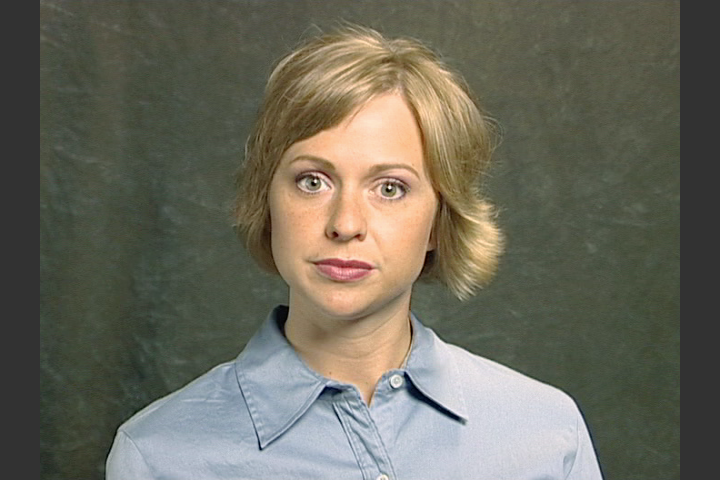
\includegraphics[width = 0.9\linewidth]{target-stimulus.png}
\caption{target stimulus}
\label{fig:target-stimulus}
\end{figure}

\begin{figure}
\centering
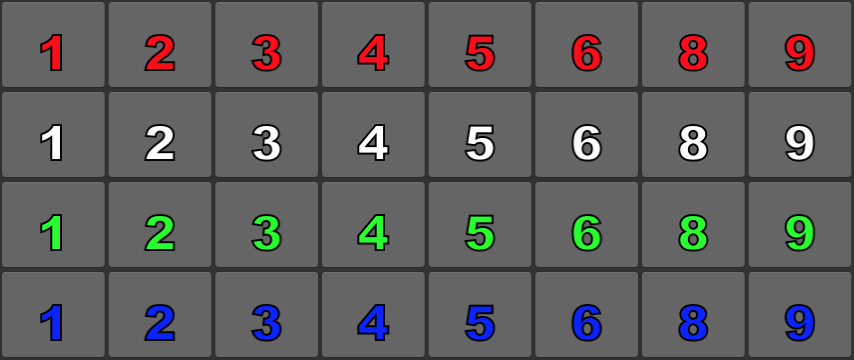
\includegraphics[width = 0.9\linewidth]{subject-response-window.png}
\caption{subject window when responding}
\label{fig:subject-response-window}
\end{figure}

\section{Output}
The results of the test are written to a plaintext file located under \texttt{\mytilde/Documents/AvSpeechInNoise Data}. The name of the file is like \texttt{Subject\_bob\_Session\_1\_Experimenter\_jim\_2020-3-13-10-30-0.txt}. The output file contains test settings and a record of trial-by-trial information. Listing~\ref{lst:example-output-file} shows an example.

\noindent\begin{minipage}{\textwidth}
\lstinputlisting[
    language=txt,
    label={lst:example-output-file},
    caption={example output file}
]{example-output.txt}
\end{minipage}

\end{document}
